% !TEX program = xelatex
% 光遗传学与视觉功能恢复 · 整合优化版（9 问 / 26 分）
% 编译：xelatex -interaction=nonstopmode -halt-on-error 本文件（跑两遍）
\documentclass[UTF8,a4paper,11pt]{ctexart}

\usepackage{geometry}
\geometry{left=1.9cm,right=1.9cm,top=2.3cm,bottom=2.3cm}
\usepackage{graphicx}
\usepackage{amsmath,amssymb}
\usepackage{booktabs}
\usepackage{longtable}
\usepackage{array}
\usepackage{enumitem}
\usepackage{xcolor}
\usepackage{caption}
\usepackage{float}
\usepackage{titlesec}
\usepackage{fancyhdr}
\usepackage[hidelinks]{hyperref}

\graphicspath{{../命题图/}{../../Resources/Downloads/原图-光遗传学视觉恢复/}}

\definecolor{deepblue}{HTML}{1F4E79}
\definecolor{deepred}{HTML}{C00000}
\definecolor{deepgreen}{HTML}{2E7D32}

\captionsetup{font=small,labelfont=bf,skip=4pt}
\titleformat{\section}{\Large\bfseries\color{deepblue}}{\thesection}{0.6em}{}
\titleformat{\subsection}{\normalsize\bfseries\color{deepblue}}{\thesubsection}{0.6em}{}
\pagestyle{fancy}
\fancyhf{}
\fancyhead[L]{\small 光遗传学与视觉功能恢复 · 整合优化版（26 分）}
\fancyhead[R]{\small\thepage}

\newcommand{\pt}[1]{\textbf{（#1分）}}
\newcommand{\lv}[1]{{\small\color{deepgreen}［#1］}}
\newcommand{\key}[1]{\textbf{\color{deepred}#1}}
\newcommand{\tian}[1]{\underline{\hspace{#1}}}
\newcommand{\choice}[1]{\par\smallskip\noindent #1\par}

\title{\bfseries 光遗传学与视网膜退化性疾病的视觉功能恢复\\[5pt]
\large 整合优化版\quad 9 问 / 26 分}
\author{}\date{2026-10-06}

\begin{document}
\maketitle
\thispagestyle{fancy}

\noindent\textbf{主线}：视网膜感光细胞损伤 → ChR2 恢复光感受 → 优化 ChR2 性能 → 优化靶细胞表达 → 检验视觉功能 → 综合评价治疗方案。
三篇论文分别承担\textbf{蛋白性能}（表1）、\textbf{细胞靶向}（表2、图2）、\textbf{整体功能评价}（表3）三个层次，共同服务于一条推理链。

\vspace{4pt}
\noindent\textbf{阅读提示}：所有专业名词均在材料或表注中给出做题所需的解释，不需要事先记忆。标"\key{命题简化}"的数据，其数值为命题需要而设定，\emph{变化趋势}依原论文改写。

\section{材料}
\addcontentsline{toc}{section}{材料}

视网膜像一台"光信号转换器"：其中的\textbf{感光细胞}（视杆细胞与视锥细胞）感受光并把光信号转变为电信号，信号再经\textbf{双极细胞}传到\textbf{神经节细胞}，由后者送往大脑皮层视觉中枢，最终形成视觉（图1）。视网膜色素变性（RP）患者的感光细胞逐渐死亡，而内层的双极细胞与神经节细胞大多存活，患者因此逐渐失明。

为让失明小鼠重新"看见"，研究者开展了以下一系列实验。

\textbf{第一步：让残存的视网膜细胞获得光感受能力。}研究者把一种来自单细胞藻类的光敏蛋白基因（\textbf{ChR2 基因}）用腺相关病毒（AAV）送入小鼠视网膜中残存的神经细胞。ChR2 蛋白能在细胞膜上形成\textbf{受光控制的离子通道}：蓝光照射时通道开放、离子流动，细胞的膜电位随之改变，从而产生电信号。由于天然 ChR2 需要较强的光才能被激活，研究者改造了 ChR2 基因中特定位置的碱基序列，获得三种突变体，并比较了它们的性能（表1）。

\textbf{第二步：让目的基因尽量只进入并表达在合适的细胞中。}基因在哪些细胞中表达、表达多少，与连接在它旁边的\textbf{调控元件}（启动子、增强子）有关：它们能影响目的基因在不同细胞中的表达水平。研究者比较了三种构建方案（方法中只有调控元件不同），结果见表2；图2 是把 ChR2 与红色荧光蛋白融合后，与能标记双极细胞的抗体共同染色的结果。

\textbf{第三步：检验视觉功能是否真的恢复。}细胞"对光有反应"不等于动物"看得见"。研究者使用\textbf{视动反应（OMR）}：把小鼠放在能显示移动条纹的装置中，若小鼠能看清条纹，其头部会随条纹运动方向转动；条纹越密集（\textbf{空间频率}越高），看清越困难，需要的光也越强。各组小鼠出现 OMR 所需的最低光强见表3。

\begin{figure}[H]
\centering
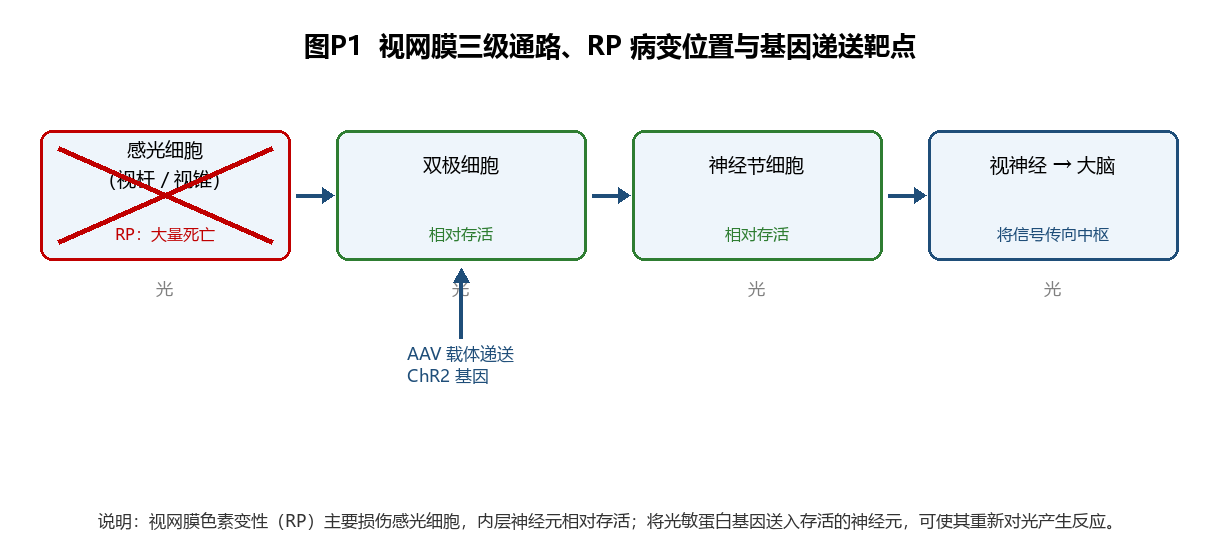
\includegraphics[width=0.64\textwidth]{P1_视网膜三级通路与病变.png}
\caption{图1\quad 视网膜三级细胞通路、RP 的主要受损环节与治疗靶点（简化示意图）}
\end{figure}

\begin{table}[H]
\centering\small
\caption*{\textbf{表1}\quad ChR2 及其突变体的性能比较（\key{命题简化}数据）}
\begin{tabular}{@{}lccc@{}}
\toprule
\textbf{变体} & \textbf{引起光响应所需的最低光强} & \textbf{光照停止后恢复到静息所需时间} & \textbf{在快速闪烁光下的响应} \\
\midrule
wt-ChR2（未改造） & 12 & 短 & 好 \\
M1（ChR2-L132C） & 5 & 中 & 中 \\
M2（ChR2-L132C/T159C） & 2 & 长 & 差 \\
M3（ChR2-L132C/T159S） & 3 & 很长 & 很差 \\
\bottomrule
\end{tabular}

\smallskip
\parbox{0.94\textwidth}{\footnotesize 注："引起光响应所需的最低光强"数值越小，表示细胞在越弱的光下即可被激活；"恢复到静息所需时间"越长，表示细胞在光照停止后越难迅速恢复，对随时间快速变化的光信号跟随能力越弱。数据为命题简化，趋势依据 Pan et al., 2014 改写。}
\end{table}

\begin{table}[H]
\centering\small
\caption*{\textbf{表2}\quad 三种构建方案的表达情况比较（\key{命题简化}数据）}
\begin{tabular}{@{}lccc@{}}
\toprule
\textbf{方案} & \textbf{ChR2 总表达量} & \textbf{双极细胞中表达比例} & \textbf{非目标细胞中表达情况} \\
\midrule
甲 & 高 & 低 & 明显 \\
乙 & 中 & 高 & 很少 \\
丙 & 低 & 很高 & 极少 \\
\bottomrule
\end{tabular}

\smallskip
\parbox{0.94\textwidth}{\footnotesize 注：三种方案的目的是相同的（让视网膜细胞获得光响应），区别只在调控元件。数据为命题简化，趋势依据 Lu et al., 2016 结果改写。}
\end{table}

\begin{figure}[H]
\centering
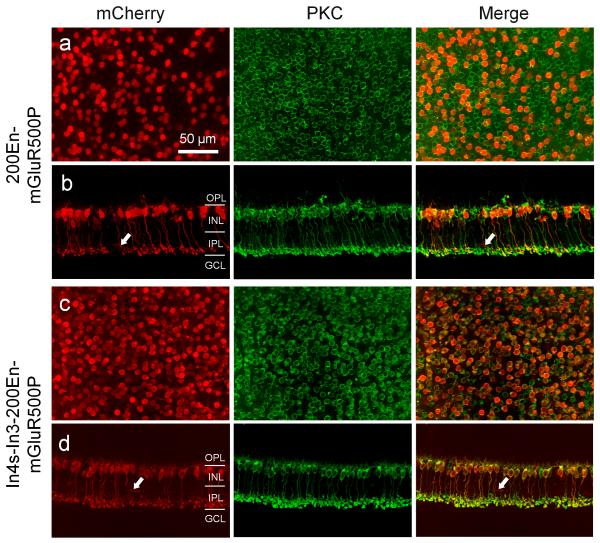
\includegraphics[width=0.58\textwidth]{Lu2016-Fig04.jpg}
\caption{图2\quad 论文原图（Lu et al., 2016）：目的基因表达产物（红）与双极细胞标记物（绿）的重叠情况}
\end{figure}

\begin{table}[H]
\centering\small
\caption*{\textbf{表3}\quad 各组小鼠出现 OMR 所需的最低光强（\key{命题简化}数据；"未出现"表示该条件下测不到 OMR）}
\begin{tabular}{@{}lccc@{}}
\toprule
\textbf{组别} & \textbf{条纹稀疏} & \textbf{条纹中等} & \textbf{条纹密集} \\
\midrule
未经基因治疗的对照组 & 未出现 & 未出现 & 未出现 \\
wt-ChR2 组 & 25 & 未出现 & 未出现 \\
M1 组 & 12 & 20 & 28 \\
M2 组 & 5 & 8 & 40 \\
M3 组 & 6 & 14 & 未出现 \\
\bottomrule
\end{tabular}
\end{table}

\section{问题（共 26 分）}
\addcontentsline{toc}{section}{问题}

\begin{enumerate}[leftmargin=2.2em,itemsep=6pt]
\item \lv{基础} \pt{2} 结合图1 与材料，RP 患者视觉功能下降的直接原因是（\quad）\\
\choice{A. 视神经被切断，信号无法上传到大脑\\
B. 感光细胞死亡，光信号无法在视网膜内被转变为神经信号\\
C. 双极细胞与神经节细胞也大量死亡，视网膜无法传递信号\\
D. 大脑皮层的视觉中枢受损，无法形成视觉}

\item \lv{基础} \pt{3} 研究者把 ChR2 基因导入残存的视网膜神经细胞后，这些细胞便能在蓝光下产生反应。请用"基因 → 蛋白质 → 细胞功能"的思路说明其原因。

\item \lv{中等} \pt{2} 据表1，说明引起光响应所需的最低光强与"光照停止后恢复到静息所需时间"之间存在怎样的总体关系；这对"应当选择怎样的变体"有什么启示？

\item \lv{拔高·数据分析} \pt{4} 表1 显示，M3 引起光响应所需的最低光强只比 M2 略高；但在表3 中，M3 在条纹中等、密集两种条件下都明显不如 M2。请结合表1 与表3 解释这一现象，并写出由此可以得到的结论。

\item \lv{中等} \pt{3}
\begin{enumerate}[label=(\arabic*),leftmargin=1.4em,itemsep=2pt]
\item 若要使目的基因\textbf{主要在双极细胞中表达}，应选择表2 中的方案\tian{0.8cm}（填"甲""乙"或"丙"）（1 分）
\item 说明你的判断理由（2 分）。
\end{enumerate}

\item \lv{拔高} \pt{3} 表2 中甲方案的 ChR2 总表达量最高，但研究者并未选择它。请结合表1—表3，说明为什么"ChR2 表达量高"不能说明视觉恢复效果好。

\item \lv{实验设计} \pt{3} 若要比较 M1 与 M2 两种变体对失明小鼠视觉功能恢复的影响，请写出该实验的\textbf{自变量}、\textbf{因变量}以及至少两个需要控制相同的变量。\tian{0.46\textwidth}

\item \lv{实验分析} \pt{2} 请回答下列两个问题（各 1 分）：
\begin{enumerate}[label=(\arabic*),leftmargin=1.4em,itemsep=2pt]
\item 为什么必须设置"未经基因治疗"的对照组？
\item 若该对照组也出现了 OMR，最可能说明什么？应如何进一步处理？
\end{enumerate}

\item \lv{拔高·综合评价} \pt{4} 有一位患者以\textbf{夜间活动为主}，且需要\textbf{躲避快速移动的物体}。请综合表1—表3 的结果，从"\textbf{变体选择}、\textbf{靶细胞表达}、\textbf{功能评价}"中至少两个方面提出你的方案，并说明依据。
\end{enumerate}

\clearpage
\section{参考答案与评分细则}
\addcontentsline{toc}{section}{参考答案与评分细则}

\begin{longtable}{@{}p{0.9cm}p{9.6cm}p{4.2cm}@{}}
\toprule
\textbf{题} & \textbf{参考答案} & \textbf{评分点} \\
\midrule
\endhead
Q1 & \textbf{B}。材料明确说明内层神经元大多存活，故 C 错；A、D 与材料中"视神经通路与视觉中枢完好"不符。 & 选 B 得 2 分，其余 0 分。 \\
\addlinespace
Q2 & 导入的 ChR2 基因在细胞内表达（转录、翻译）出 ChR2 蛋白；该蛋白分布到细胞膜上，形成能被蓝光控制的离子通道；蓝光照射时通道开放、离子流动，使细胞的\textbf{膜电位发生改变}，细胞因此产生电信号（光响应）。 & 基因表达出 ChR2 蛋白 1 分；蛋白分布到细胞膜并形成受光控制的通道 1 分；蓝光→离子流动→膜电位改变→产生电信号 1 分。缺少"膜电位改变／产生电信号"扣 1 分。 \\
\addlinespace
Q3 & \textbf{总体关系}：引起光响应所需的最低光强越低（细胞越容易被弱光激活）的变体，光照停止后恢复到静息所需的时间总体越长（wt→M1→M2 的趋势）；但二者并非严格对应——M3 所需光强略高于 M2，恢复时间却更长。\textbf{启示}：提高"对弱光的敏感性"往往要付出"时间响应变慢"的代价，因此选择变体不能只看光敏性，还要看它对随时间变化的光信号的分辨能力。 & 指出总体关系（越易被弱光激活→恢复越慢）1 分；指出并非严格对应，或得出"不能只看光敏性、须兼顾时间响应"1 分。 \\
\addlinespace
Q4 & \textbf{解释}：M3 与 M2 被弱光激活的能力接近（所需最低光强 3 与 2），说明两者在"能否被弱光激活"上差别不大；差别在于\textbf{时间响应}——M3 光照停止后恢复到静息所需时间最长（表1），对随时间快速变化的光信号跟随能力最差。表3 中用移动条纹进行测试，条纹越密集，要求细胞跟随光强变化的速度越快，因此 M3 在条纹中等、密集时不能稳定引起 OMR（14、"未出现"），而 M2 为 8、40。\textbf{结论}：当两种变体的光敏性接近时，\textbf{时间响应特性成为决定视觉功能恢复效果的关键}；仅根据光敏性（或表达量）判断恢复效果是不充分的，必须结合行为水平的整体功能评价。 & 指出两者被弱光激活的能力接近 1 分；用"恢复时间长→跟随能力差"作出机制解释 1 分；把"条纹密集需要更快的跟随"与结果联系起来 1 分；得出"光敏性相近时时间响应成为关键／不能只看单一指标"的结论 1 分。 \\
\addlinespace
Q5 & (1) \textbf{丙}。(2) 丙方案在目标细胞（双极细胞）中的表达比例最高、在非目标细胞中表达极少，说明目的基因被尽量限制在双极细胞中表达，\textbf{细胞特异性最好}；甲方案虽然总表达量最高，但在非目标细胞中表达明显，不能达到"主要在双极细胞中表达"的目的。 & (1) 填"丙"1 分。(2) 依据"双极细胞中表达比例最高"1 分；依据"非目标细胞中表达极少（特异性好）"或"指出甲的高表达量不等于特异性"1 分。 \\
\addlinespace
Q6 & 不充分。①"ChR2 总表达量"只说明细胞内产生了多少 ChR2 蛋白，属于\textbf{蛋白质水平}的信息；② 甲方案虽总表达量最高，但它在非目标细胞中表达明显（表2），这些细胞即使产生 ChR2，也未必形成有效的视觉信号，还可能干扰视网膜原有的信号处理；③ 表1、表3 表明，即使表达了蛋白，若其\textbf{时间响应特性差}（如 M3），动物在行为上仍可能测不到 OMR。因此从蛋白质水平→细胞水平→行为（功能）水平存在层次差异，视觉恢复效果最终必须由\textbf{行为学功能指标}来评价。 & 指出表达量属蛋白质水平、是必要而非充分条件 1 分；结合表2（表达位置、非目标细胞）说明 1 分；结合表1／表3（时间响应→行为表现）或明确"须以行为学功能为最终评价标准"1 分。 \\
\addlinespace
Q7 & \textbf{自变量}：导入的 ChR2 变体种类（M1 或 M2，并设置未经相同基因治疗处理的对照组）。\textbf{因变量}：是否出现 OMR、出现 OMR 所需的最低光强。\textbf{需控制相同的变量}（答出两个）：小鼠的遗传背景与生理状态（同一个失明模型，处理部位与方式一致）、注射的载体量与浓度、注射后至测定的时间、条纹的移动速度与光刺激条件等。 & 自变量 1 分（须体现"不同变体"且含对照）；因变量 1 分；控制变量答出两个 1 分。 \\
\addlinespace
Q8 & (1) 排除"失明小鼠自身残留的光感受能力、注射操作或光刺激"等因素也能引起 OMR 的可能，从而说明观察到的 OMR\textbf{确实由导入的 ChR2 引起}，使因果判断成立。(2) 说明该反应不是（或不只是）由导入的 ChR2 引起的——可能小鼠并未真正失去光感受能力（模型不纯），也可能是 OMR 的判定标准过宽或有其他因素干扰；此时应先检验小鼠是否确实失去光感受能力，并重新设定判定标准后再作结论。 & (1) 排除其他因素、证明因果 1 分。(2) 指出"反应并非由 ChR2 引起／模型可能不纯"0.5 分，提出"先检验模型、再重设判定标准"0.5 分。 \\
\addlinespace
Q9 & \textbf{（示例，答出"两个方面＋依据"即可）}\newline
\textbf{① 变体选择}：夜间活动需要"弱光下即可被激活"，表3 中 M2 在条纹稀疏、中等时所需光强最低（5、8），最符合夜间使用；但 M2 恢复到静息所需时间最长，在条纹密集（对应快速移动的物体）时所需光强反而高于 M1（40 与 28），说明它分辨快速移动物体的能力较弱。因此若患者最看重辨识快速移动物体，可考虑 M1；若最看重夜间看清环境，可考虑 M2。\newline
\textbf{② 靶细胞表达}：应选择表2 中丙（或乙）方案，使 ChR2 尽量只在双极细胞中表达，减少非目标细胞的表达及其对原有信号的干扰。\newline
\textbf{③ 功能评价}：不能只用一种条件评价疗效，应同时测定条纹稀疏与密集条件下的 OMR，并增加如瞳孔对光收缩等其他指标。\newline
\textbf{结论}：视觉恢复需要综合考虑\textbf{对弱光的敏感性、时间响应、靶细胞表达、非靶细胞表达以及行为水平的功能表现}，不能仅凭单一指标（如光敏性或表达量）判断优劣。 & 结合"夜间（弱光）"与"移动物体（快速变化）"两个需求并引用表3 的具体数据 1 分；指出 M2 与 M1 之间的取舍关系（弱光与快速分辨不能兼得）1 分；从至少两个方面提出方案且合理 1 分；明确得出"需综合多指标、单一指标不足以判断"的结论 1 分。 \\
\bottomrule
\end{longtable}

\noindent\textbf{难度分层}：基础 5 分（Q1、Q2）；中等 8 分（Q3、Q5、Q7）；拔高 13 分（Q4、Q6、Q8、Q9）。\textbf{主要区分点}：Q4（解释"光敏性接近而功能差异明显"）、Q6（蛋白质—细胞—行为三个层次）、Q9（多指标综合决策）。

\section*{命题设计说明（供教师参考）}
\addcontentsline{toc}{section}{命题设计说明}

\begin{enumerate}[leftmargin=1.8em,itemsep=3pt]
\item \textbf{一条主线、三篇论文分层}：三篇论文不再各自成题，而分别承担"蛋白性能（表1）—细胞靶向（表2、图2）—整体功能评价（表3）"三个层次，全题沿"损伤 → 恢复光感受 → 优化性能 → 优化表达 → 检验功能 → 综合评价"单向推进。
\item \textbf{连续设问}：Q3 的结论（光敏性与时间响应存在权衡）是 Q4 解释数据的前提；Q4 的结论（时间响应影响功能）是 Q6、Q9 的依据；Q5 的选择结论（丙方案特异性最好）被 Q9 直接使用。
\item \textbf{数据刻意"不规律"}：① 表1 中"最低光强"与"恢复时间"总体相关但并非严格单调（M3 光强略高于 M2、恢复时间却更长）；② 表2 中甲的总表达量最高但特异性最差，没有哪个方案在所有指标上都最优；③ 表3 中 M2 在条纹稀疏、中等时最好，在条纹密集时却不如 M1——形成\textbf{交叉}，避免"一眼看出答案"。
\item \textbf{减少记忆型设问}：全题没有"某物质是什么""某技术是什么"的提问；所有设问均为"据表说明关系""解释现象""说明理由""设计方案""综合评价"。
\item \textbf{科学表述的把关}：材料与答案一律表述为"调控元件\textbf{影响}目的基因在不同细胞中的表达水平"（而非"决定细胞类型"）；一律表述为"通道开放、离子流动，\textbf{膜电位发生改变}，从而产生电信号"（未把 ChR2 开放等同于产生动作电位）。
\item \textbf{实验思想为主}：Q7、Q8 只考查自变量、因变量、控制变量与对照的作用及异常结果的分析，不涉及病毒载体构建、启动子序列等专业操作细节。
\end{enumerate}

\section*{附录\quad 论文原图对照（课堂延伸用）}
\addcontentsline{toc}{section}{附录：论文原图对照}

\begin{figure}[H]
\centering
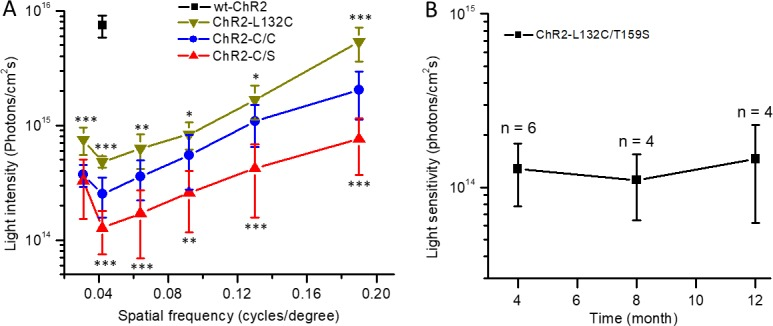
\includegraphics[width=0.72\textwidth]{Lu2018-Fig04.jpg}
\caption{图A\quad 论文原图（Lu et al., \textit{IOVS}, 2018, Fig.~4）：三种 ChR2 变体的 OMR 阈值光强—空间频率关系，与表3 的设计思路一致，供课堂延伸或按真实数据替换表3 时对照使用。}
\end{figure}

\noindent\small 全部 22 张论文原图与三篇文献存于 \texttt{00 - Personal/Resources/Downloads/}。

\end{document}
